\section{GPU Computing}
\label{sec:gpuComputing}

\subsection{Introduction}

Advances in computer graphics and the growth of the video game industry lead to the development of powerful GPUs in the past ten years. It's worth noting that the video game industry generates more revenue than Hollywood nowadays \cite{videogamesRevenue}. While early GPUs were designed to accelerate a fixed graphics pipeline controlled from the CPU, modern GPUs are fully programmable giving the programmer control of the graphics pipeline and allow the execution of small programs, called shaders, directly on the GPU. Developers soon realized that this computing power cannot just be used for graphics, but also to accelerate many problems in computational science. With the release of CUDA in 2007 it became practical to develop computational intense applications for GPUs. Since then thousands of works have been published in which GPUs are used to accelerate computing.

The next two chapters give a short overview of the GPU architecture and the framework used to program GPUs in order to understand the rest of the thesis. For an extensive introduction to GPU programming the author recommends the book  ''Programming Massively Parallel Processors: A Hands-on Approach'' by David B. Kirk and Wen-mei W. Hwu \cite{cudabook} as well as the CUDA C programming guide \cite{cudaguide} which comes with the CUDA software development kit.

\subsection{Architecture of Modern GPUs}
\label{sec:gpuArch}

The performance of modern hardware is largely constrained by the latency of dynamic random access memory (DRAM). While the performance of processors increased greatly, latency of DRAM access did not decrease much, this is often referred to as the memory wall. The reason for this lies in the way how DRAM works: DRAM is basically a very large array of tiny semiconductor capacitors. The presence of a tiny amount of electrical charge distinguishes between 0 and 1. To read the data the charge must be shared with a sensor and if a sufficient amount of charge is present, the sensor detects a 1 (0 otherwise). This is a slow process\footnote{Furthermore DRAM cells must be periodically refreshed otherwise they loose their charge. During refresh cycles the data cannot be accessed.}, the latency for a global memory access is around 400 to 800 clock cycles \cite[5.2.3]{cudaguide} on a GPU.  Modern DRAMs use a parallel process to increase the rate of data: Each time a location is requested many consecutive locations, which include the requested location, are read. Data at consecutive locations can be read at once and then be transferred at high speed to the processor. The programmer must ensure that the program arranges its data in a way that it can be accessed consecutively whenever possible. Otherwise the application will not perform optimally, because more memory transactions than theoretically needed will be executed.

While CPUs are kept busy by using complex automatic caching mechanism\footnote{Around $\frac{1}{3}$ of all transistors are just used for caching in a modern CPU.}, GPUs hide latency using massive parallelism: Thread scheduling on GPUs is implemented in hardware: Each streaming multiprocessor (SM) has its own scheduler. The scheduler bundles threads into warps which are executed simultaneously. If a warp has to wait for data it can be exchanged with another warp ready for calculations. Because scheduling is implemented in hardware dispatching and switching warps has negligible overhead. The SM can automatically coalesce memory access, which is how to the high memory bandwidth advertised \cite[Figure 1.1]{cudaguide} is achieved: If multiple threads in the same warp access consecutive memory locations at the same time hardware coalesces this into a single memory transaction \cite[Appendix F 3.2.1]{cudaguide}. Further vectorized loading of fundamental data types is supported \cite[Table 86]{ptxMan}.

Figure \ref{gfx:fermi} illustrates Nvidia's current architecture named after the Italian physicist Enrico Fermi. Fermi is Nvidia's second generation architecture which supports CUDA. The figure shows a single streaming multiprocessor. The GeForce GTX 470, for example, has 14 multiprocessors and each one has 32 cores\footnote{This explains the warp size of 32.}. The register file is shared among all the threads assigned to an SM. Each thread has it's own register state and program counter, threads can therefore branch independently. However since a warp executes one common instruction at time divergent branching in a wrap is inefficient. Data dependent branches may lead to threads taking different execution paths. In this case both parts a branch are executed sequentially with the concerning threads disabled in either branch \cite[Chapter 4.1]{cudaguide}. Kernels (a program executed on the GPU, see chapter \ref{sec:cuda}) with high register usage limit the number of blocks CUDA can assign to one SM, this may result in poor performance because the scheduler has too few warps to keep the SM busy. To calculate the occupancy of a CUDA program Nvidia provides a spreadsheet \cite{occupancySpreadsheet}. GPUs are often called SIMD (single instruction multiple data) architectures. However compared to SIMD architectures such as Intels SSE (streaming SIMD extension) a GPU offers much more: A scheduler implemented in hardware, state for each threads, independent branching (affects performance, but possible), shared memory, etc. Because of this Nvidia refers to their architecture as \emph{SIMT (single instruction multiple threads)}.

\begin{figure}[H]
  \centering
  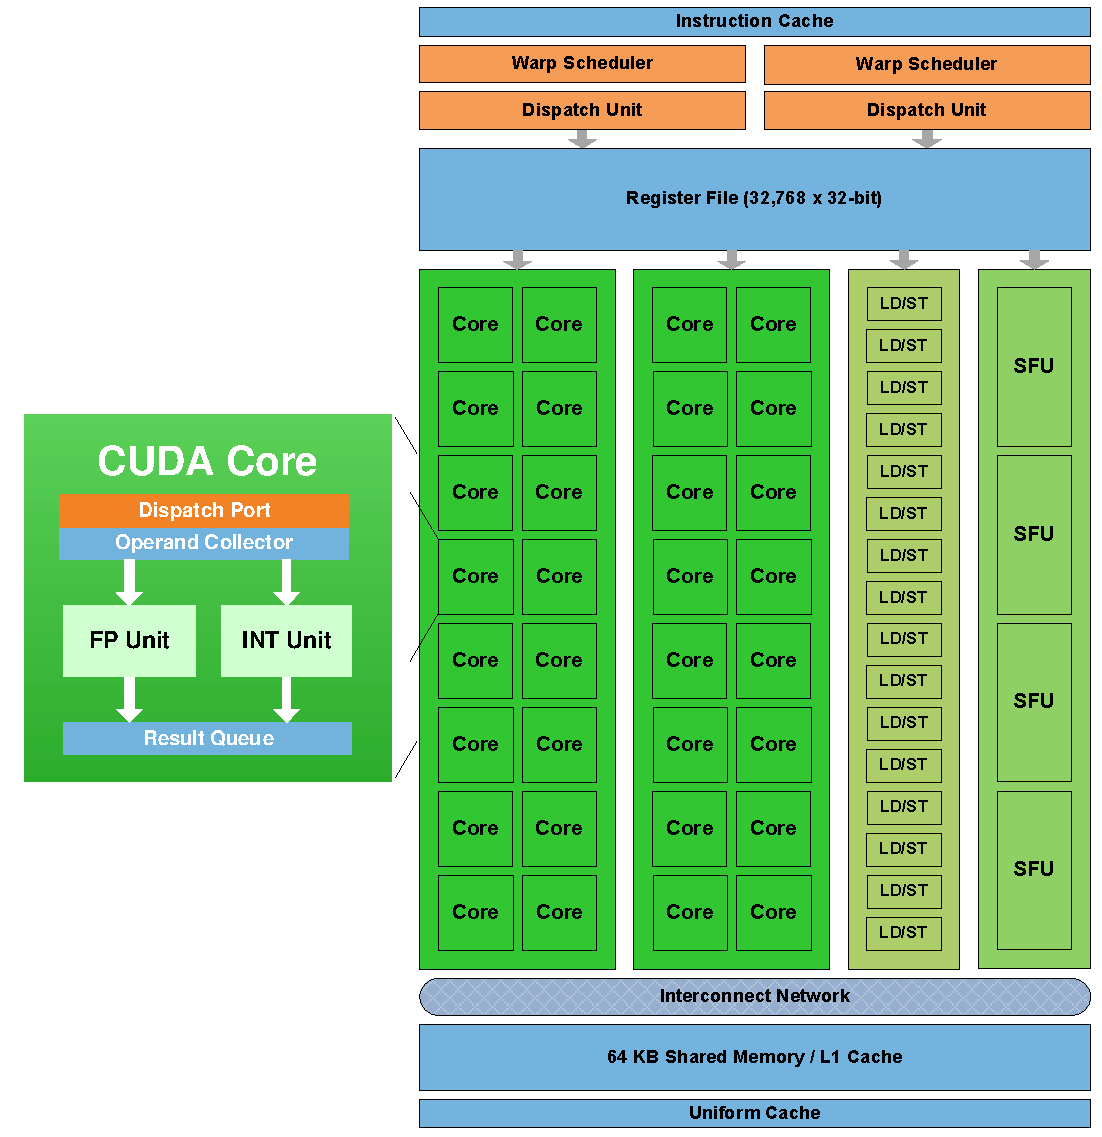
\includegraphics[scale=0.6]{content/gfx/FermiArch.pdf}
  \caption{Nvidia's Fermi architecture, taken from \cite{fermiWhitepaper}.}
  \label{gfx:fermi}
\end{figure}

\subsection{CUDA}
\label{sec:cuda}

CUDA stands for Compute Unified Device Architecture and is a C-style API to program Nvidia's hardware. CUDA is scalable, which means programs written in CUDA can run on any CUDA enabled GPU, independent of the exact hardware configuration. For example the same program can run on a GPU with two streaming multiprocessors or on one with four or eight multiprocessors. However when it comes to performance optimization knowledge of the underlying hardware is often still required.

CUDA defines three key abstractions - a hierarchy of \textbf{thread groups}, \textbf{shared memory} and \textbf{barrier synchronization}. The CUDA terminology differentiates between the host as the CPU executing a host program sequentially and the device (usually a GPU) which executes the CUDA program in parallel. A CUDA host program can allocate memory on the device, copy data between the host and the device and execute programs on the GPU. Programs running on the GPU are called \textbf{kernels}. A kernel must be configured when it is called, meaning that the programmer must specify on how many threads blocks the kernel runs and the number of threads per block. Kernels are defined and invoked using a proprietary syntax \cite[2.1]{cudaguide}. CUDA source files usually end with \verb+cu+ and can include a mix of host and device code. During the compilation workflow the host code is separated from the device code. The device code is compiled into assembly form, and the host code is passed on to the concerning compiler (for example \verb+g+++ on a Linux environment) \cite[3.1]{cudaguide}.